\section{Related Work}
\subsection{Fairness Metrics}
A common mode of evaluation for fairness with respect to a sensitive variable is defined as the Equality of Odds. \cite{HardtPS16} 
\begin{definition}
\textbf{Equality of Odds} We say that a predictor $\hat{Y}$ satisfies equalized odds with respect to protected attribute $A$ and outcome $Y$, if $\hat{Y}$ and $A$ are independent conditional on $Y$.

\[  P(\hat{Y}=\hat{y}|Y=y, A=m) = P(\hat{Y}=\hat{y}|Y=y, A=n) \]
\[\forall Y, \forall m,n \in A \]

\end{definition}
This paper will explicitly utilize this metric as a standard for evaluation.

\subsection{Survey Comparison of Fairness Aware Methods}

Beutel ~\cite{Beutel2017DataDA} models the problem of debiasing as a multi-task learning problem where the model is trained to predict the output label and is  penalized if the same shared hidden layers of a feedforward neural network can be used to predict the sensitive variable accurately. The problem formulation differs from than the goals of predictive equality and avoiding disparate impact that we are seeking to achieve in our study. In their adversarial approach, the gradients are propagated such that the model is penalized when it predicts the correct sensitive variable and likewise the model is trained to predict the opposite (in case of a binary sensitive variable) of the true label. One potentially pitfall is the model could result in propagating the bias in the model, albeit in the reverse direction.

Zhao ~\cite{Zhao2017MenAL} aims to achieve corpus level parity for each of the outcomes in a classification setting. They do so by introducing Lagrangian relaxation after each iteration of the classification training. This implies that updates are approximations on each sample in the goal of achieving corpus level parity across sensitive variables. While theoretically this approach can scale to multiple bias features, the empirical behavior for the rate of convergence of the combined loss optimization of the Lagrangian approximation has not been extensively explored.

Menon and Williamson ~\cite{Menon2018TheCO} show that a disparate impact constraint is equivalent to a cost sensitive
constraint, i.e. their super-level sets are equivalent.  Similarly, they demonstrate for the mean difference (MD) score, the corresponding balanced cost sensitive risk has a cost-parameter that does not depend on $\tau$ (the MD constraint). They also formulate a fairness frontier: for a given lower bound on fairness, it measures the best excess risk over the solution without a fairness constraint. They give the theoretical limitation from which the trade-off between fairness and accuracy stems, that is dependent on the data, but not any classifier.

Kleinberg ~\cite{Kleinberg2017PlanningWM} considers two biases based on planning (present bias and sunk cost bias) and formulates the reward such that it is parameterized by (b,T) denoting the modification it makes to the final perceived reward at each step. Examples show that behaving naively or in sophisticated manner about one or both of these biases might be optimal in different conditions. The remainder of the paper isn't directly applicable to this work as it is defined as a path finding problem where rewards are adjusted by different biases and defining those parameters can be difficult.

Pleiss ~\cite{Pleiss2017} and  Raghavan ~\cite{Raghavan2018TheEO} proves that equality of odds can't be achieved by two models on separate groups which are calibrated (i.e the classification probabilities have a meaning relevant to the population), unless both the models achieve perfect accuracy. The work derives a generalized impossibility result that shows that satisfying equalized odds for more than one cost functions which capture FNR/FPR is infeasible. Empirically, they show the impact of imposing calibration and an equal cost constraint on real-world datasets. In many cases, this will result in performance degradation, while simultaneously increasing other notions of disparity.

\subsection{Potential Weaknesses with Current Fairness Metrics}

In this paper we begin to address the following possible issues with imposing fairness constraints on sensitive variables. 
% * <ananthbalashankar@gmail.com> 2018-08-21T13:46:19.689Z:
% 
% We don't address some of these in the paper, especially the first two.
% 
% ^.
\begin{enumerate}
	
	\item Impossibility Result for optimizing for Accuracy Across Sensitive Subgroups to be incompatible with Optimizing for FP and FN rates individually as shown in Figure \ref{impossibility}.
	\item Hard constraints even with relaxation factor can cause inequity across subgroups : Equality of odds cant be achieved by two models on separate groups when calibrated. 
    \item Effects of variations in prevalence and statistics across subpopulations 
    \item Confounding Factors can drastically alter interpretation of fairness across sensitive variables and without their inclusion, we may degrade performance and cause further inequity in supervised learning tasks.
\end{enumerate}

\subsection{Pareto-Efficiency}
	We seek to mitigate some of the weaknesses described above by employing Pareto-Efficiency or Pareto Optimality, an established concept in economics, engineering and life sciences.
    
\begin{definition}
\textbf{Pareto Efficiency} is a state where resources are allocated in which it is impossible to redistribute resources to make any one criterion or party better off without making another criterion worse off. 
\end{definition}

Pareto-efficiency has been extensively studied in defining trade-offs between optimizations of multiple objectives. With respect to fairness, \cite{paretoTradeoff} explores the Pareto optimality between overall accuracy and violation of fairness constraints. Although such a comparison is important and in many cases necessary by a domain expert, it is a measure of two separate metrics and needs to be carefully evaluated. In our work, we focus on the trade-offs between the performance of various subgroups which are comparable and hence the trade-offs can be easily evaluatedm simultaneously on the Pareto-optimal curve. However, in \cite{LiptonEnvyFree}, it was proved that achieving an envy free (fair) allocation of indivisible resources is a co-NP complete problem and as such we need to explore heuristic based algorithms. Study of subgroup specific performance and use of transfer learning like methods have been explored through decoupling in \cite{pmlr-v81-dwork18a}.

\begin{figure*}[htbp]
	\begin{center}
		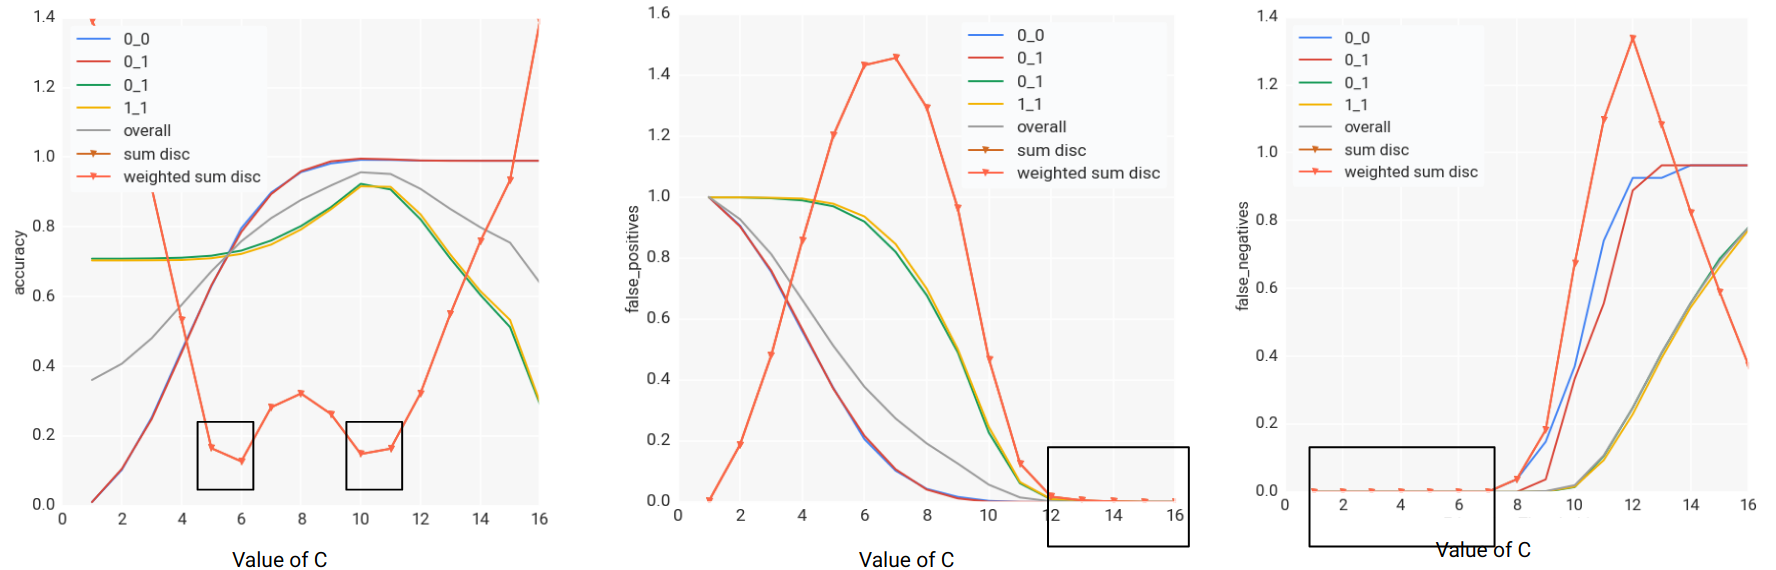
\includegraphics[width=7in,height=2.2in]{impossibility.png} 
        \setlength{\belowcaptionskip}{-8pt} 
		\caption{Example showing impossibility to equalize accuracy, FPR and FNR at the same time}
		\label{impossibility}
	\end{center}
\end{figure*}
